\renewcommand{\d}{\mathrm d}
\subject{ESPResSo Tutorial}
\title{The GPU Electrokinetics Method in \ES{}:
Electroosmotic Flow
} %\author{ Georg Rempfer \thanks{\ttfamily georg@icp.uni-stuttgart.de}}
\date{\today}
\publishers{Institute for Computational Physics, University of Stuttgart}
\maketitle 
\begin{center}
  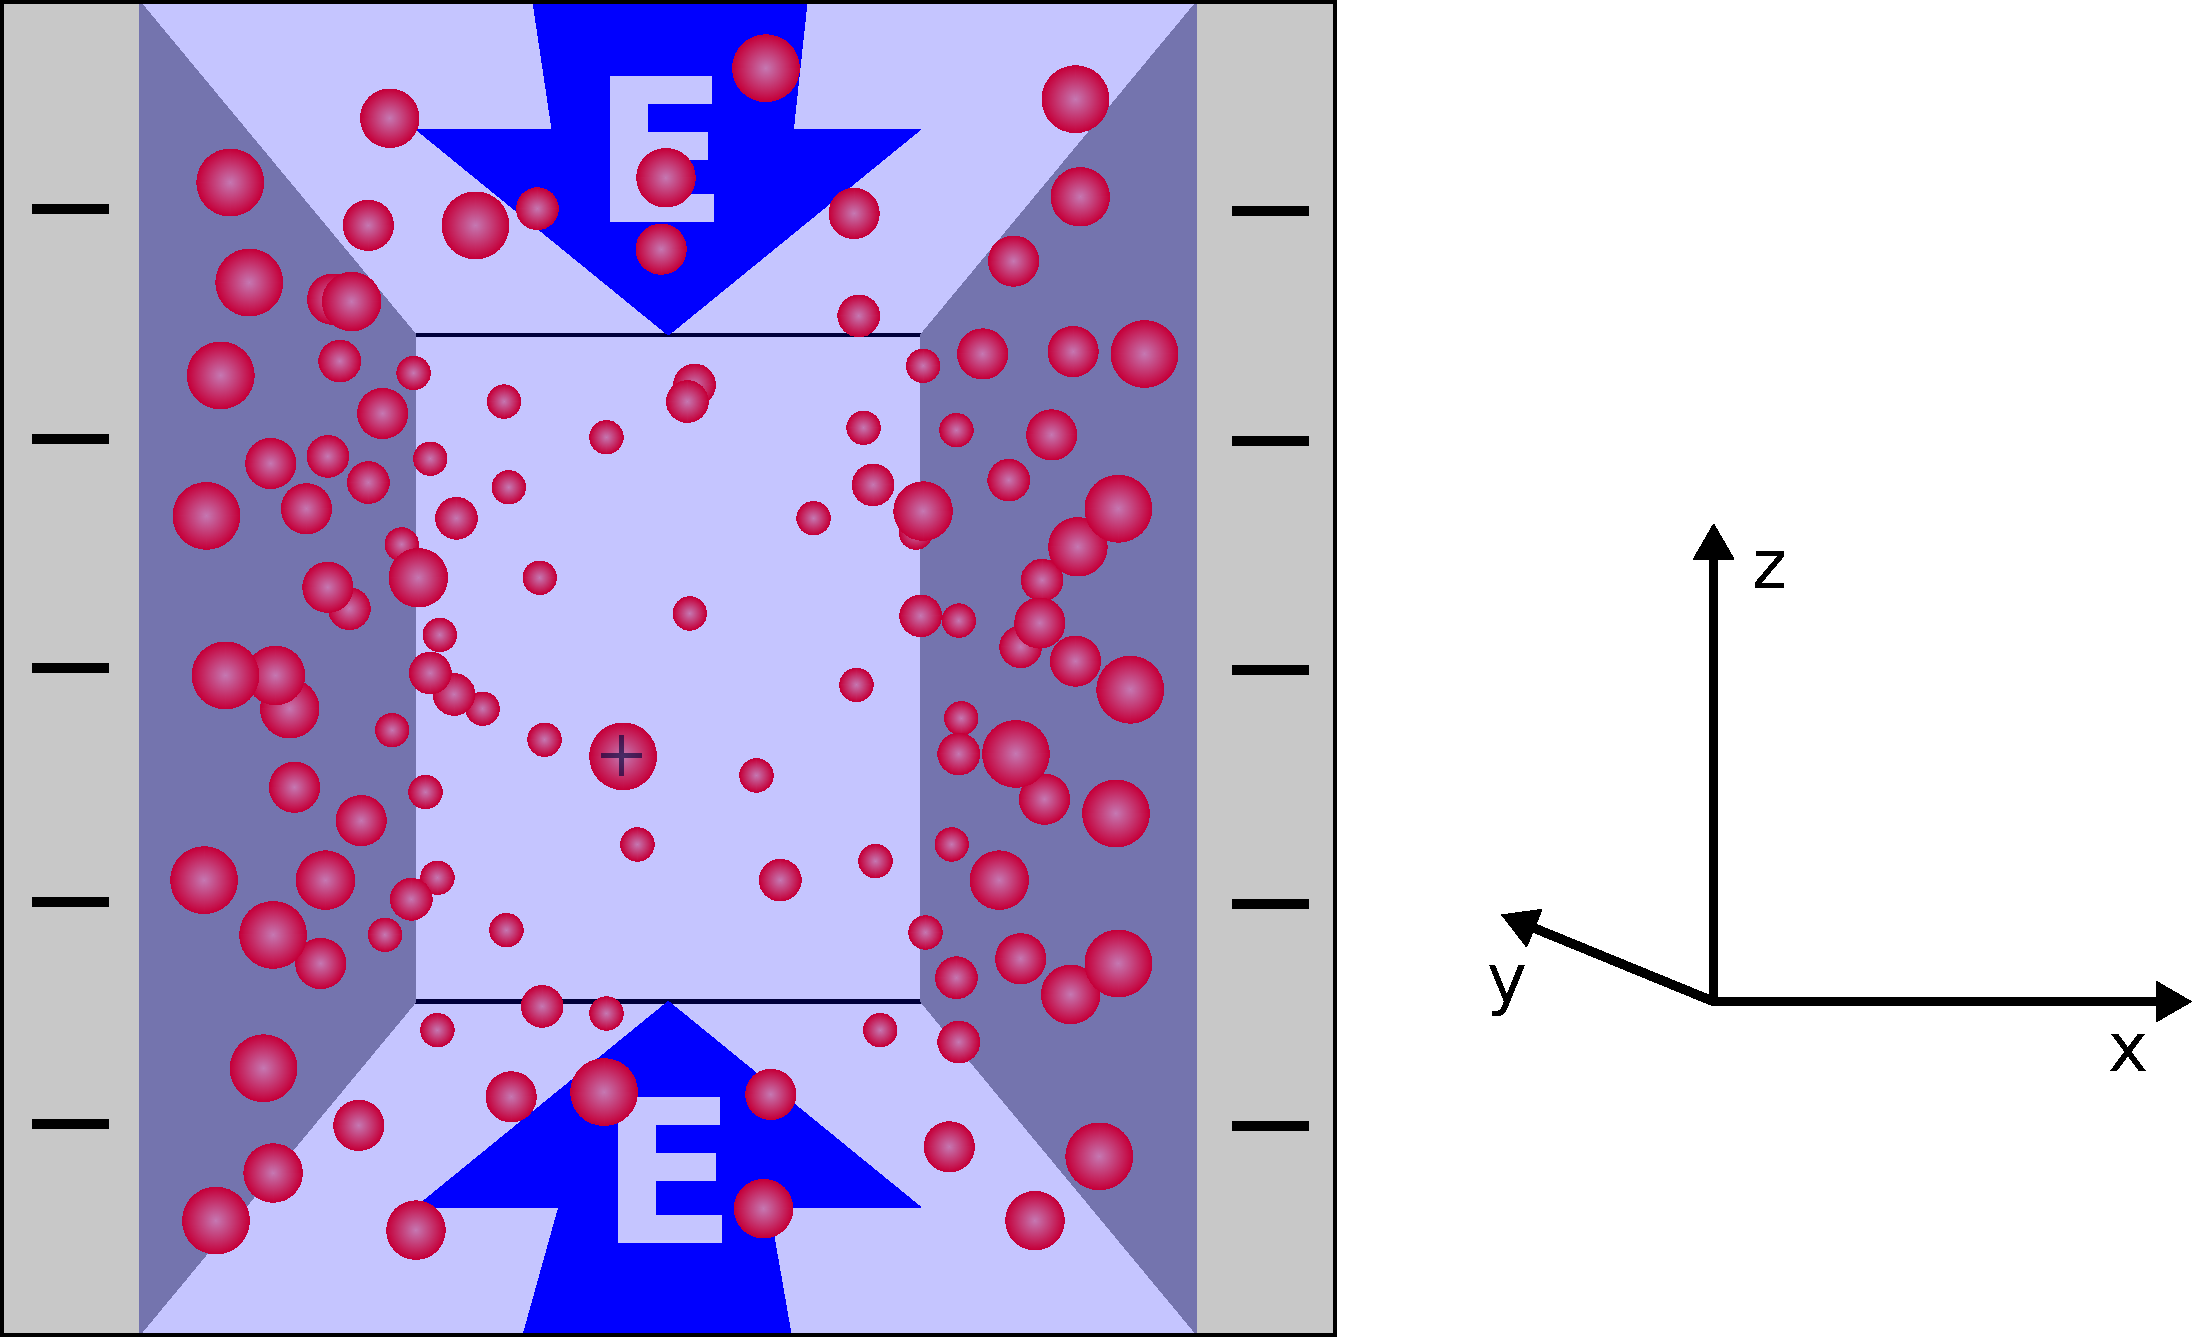
\includegraphics[width=0.7\columnwidth]{figures/schlitzpore_3d.pdf}
\end{center}
\pagebreak
\definecolor{mygray}{gray}{.75}
%\begin{center}
%  \colorbox{mygray}{ 
%\begin{minipage}[h]{13cm}
%  {\bf \large Before you start:}\\
%  With this tutorial you can get started using the Electrokinetics method
%  for scientific applications. We give a brief introduction about the theory
%  and how to use it \ES{}. 
%  We have selected one sample problem for which an analytic solution exists.
%\end{minipage}
%}
%\end{center}

 \tableofcontents
 \pagebreak
  
\section{Introduction}

%\floatingBox{5}{4cm}{Mein Text der in der Box abgebildet werden soll. Mal schauen wie das klappt.} 

In recent years the lattice-Boltzmann method (LBM) has proven itself to be a viable way to introduce hydrodynamic interactions into coarse-grained MD simulations with moderate computational cost. The success of the GPU LBM implementation in \ES{} and similar developments in other software packages created demand for further developments in this area. \ES{} features two such algorithms, namely ELECTROHYDRODYNAMICS, and ELECTROKINETICS (EK). Both of these make use of the LBM and extend it to coarse-grain not only the solvent molecules but also ionic solutes. ELECTROHYDRODYNAMICS does so using a slip layer coupling for charged particles valid in the thin Debye layer (large salt concentration) limit\cite{hickey10a}, while EK explicitly treats the ionic solutes in a continuum fashion and is valid for a wide range of salt concentrations\cite{capuani04a,rempfer13a,rempfer16a}.

\subsection*{Tutorial Outline}

To make our first steps using ELECTROKINETICS we will work on one of the few systems for which analytic solutions for the electrokinetic equations exist -- the slip pore geometry with a counterion-only electrolyte. The same slit pore system is also treated in the LBM tutorial, but there, the ionic species were modeled as explicit particles. For this system, the two approaches lead to exactly the same results~\cite{rempfer10a}. Differences are only becoming significant for multivalent ions, very high salt concentrations, and very high surface charge, since then the mean-field approach the EK is employing, basically solving the Poisson-Nernst-Planck formalism plus the Navier-Stokes equation on a lattice, gives significantly different results from explicit ion approaches \cite{deserno00a,holm01a,deserno01c}.

This tutorial is divided into three sections. The first section~\ref{sec:theory} introduces the electrokinetic equations and the analytical solution for the slit pore system, while the second section~\ref{sec:simulation} deals exclusively with the simulation, its setup, and the results.

If you already know about simple diffusion-migration-advection equations, continuum electrostatics, and Navier-Stokes, then you can skip the first section.

\pagebreak
